\documentclass{article} % \documentclass{} is the first command in any LaTeX code.  It is used to define what kind of document you are creating such as an article or a book, and begins the document preamble

\usepackage{amsmath} % \usepackage is a command that allows you to add functionality to your LaTeX code
\usepackage{graphicx}
\graphicspath{ {./images/} }
\title{Efficient Computation of the DFT: FFT Algorithms} % Sets article title
\author{Hunter Mills} % Sets authors name
\date{\today} % Sets date for date compiled

% The preamble ends with the command \begin{document}
\begin{document} % All begin commands must be paired with an end command somewhere
    \maketitle % creates title using information in preamble (title, author, date)
    These notes will only cover sections 8.1.1 and 8.1.3.\\
    
    \section{Efficient Computation of the DFT: FFT Algorithms} % creates a section
	The computational problem for the DFT is to compute the sequence $K(k)$ of $N$ complex numbers given $x(n)$. For each value of $k$ the DFT involves $N$ complex multiplies and $N-1$ complex additions which gives the algorithms $O(N^2)$. The two properties that are levarged are the symmetry property and the periodicity property.
	\begin{equation}
	\text{Symmetry : } W_N^{k+N/2} = -W_N^k
	\end{equation}
	\begin{equation}
	\text{Periodicity : } W_N^{k+N} = W_N^k
	\end{equation}
	
	\section{Radix-2 FFT Algorithms}
	These algorithms are derived in the book pg 520. I will include figures and important equations here. The first figure shows when you only split the DFT sum into two parts but it can continually be split until the resulting sequences are reduced to one point sequences. 
	\subsection{Decimation in Time}
	\begin{equation}
	f_1(n) = x(2n)
	\end{equation}
	\begin{equation}
	f_2(n) = x(2n + 1)
	\end{equation}
	
	Figure 1 shows the first step in the Radix 2 algorithm when you split the DFT into two terms. This is the decimation in time version. 
	
	\begin{figure}[h]
	\centering
	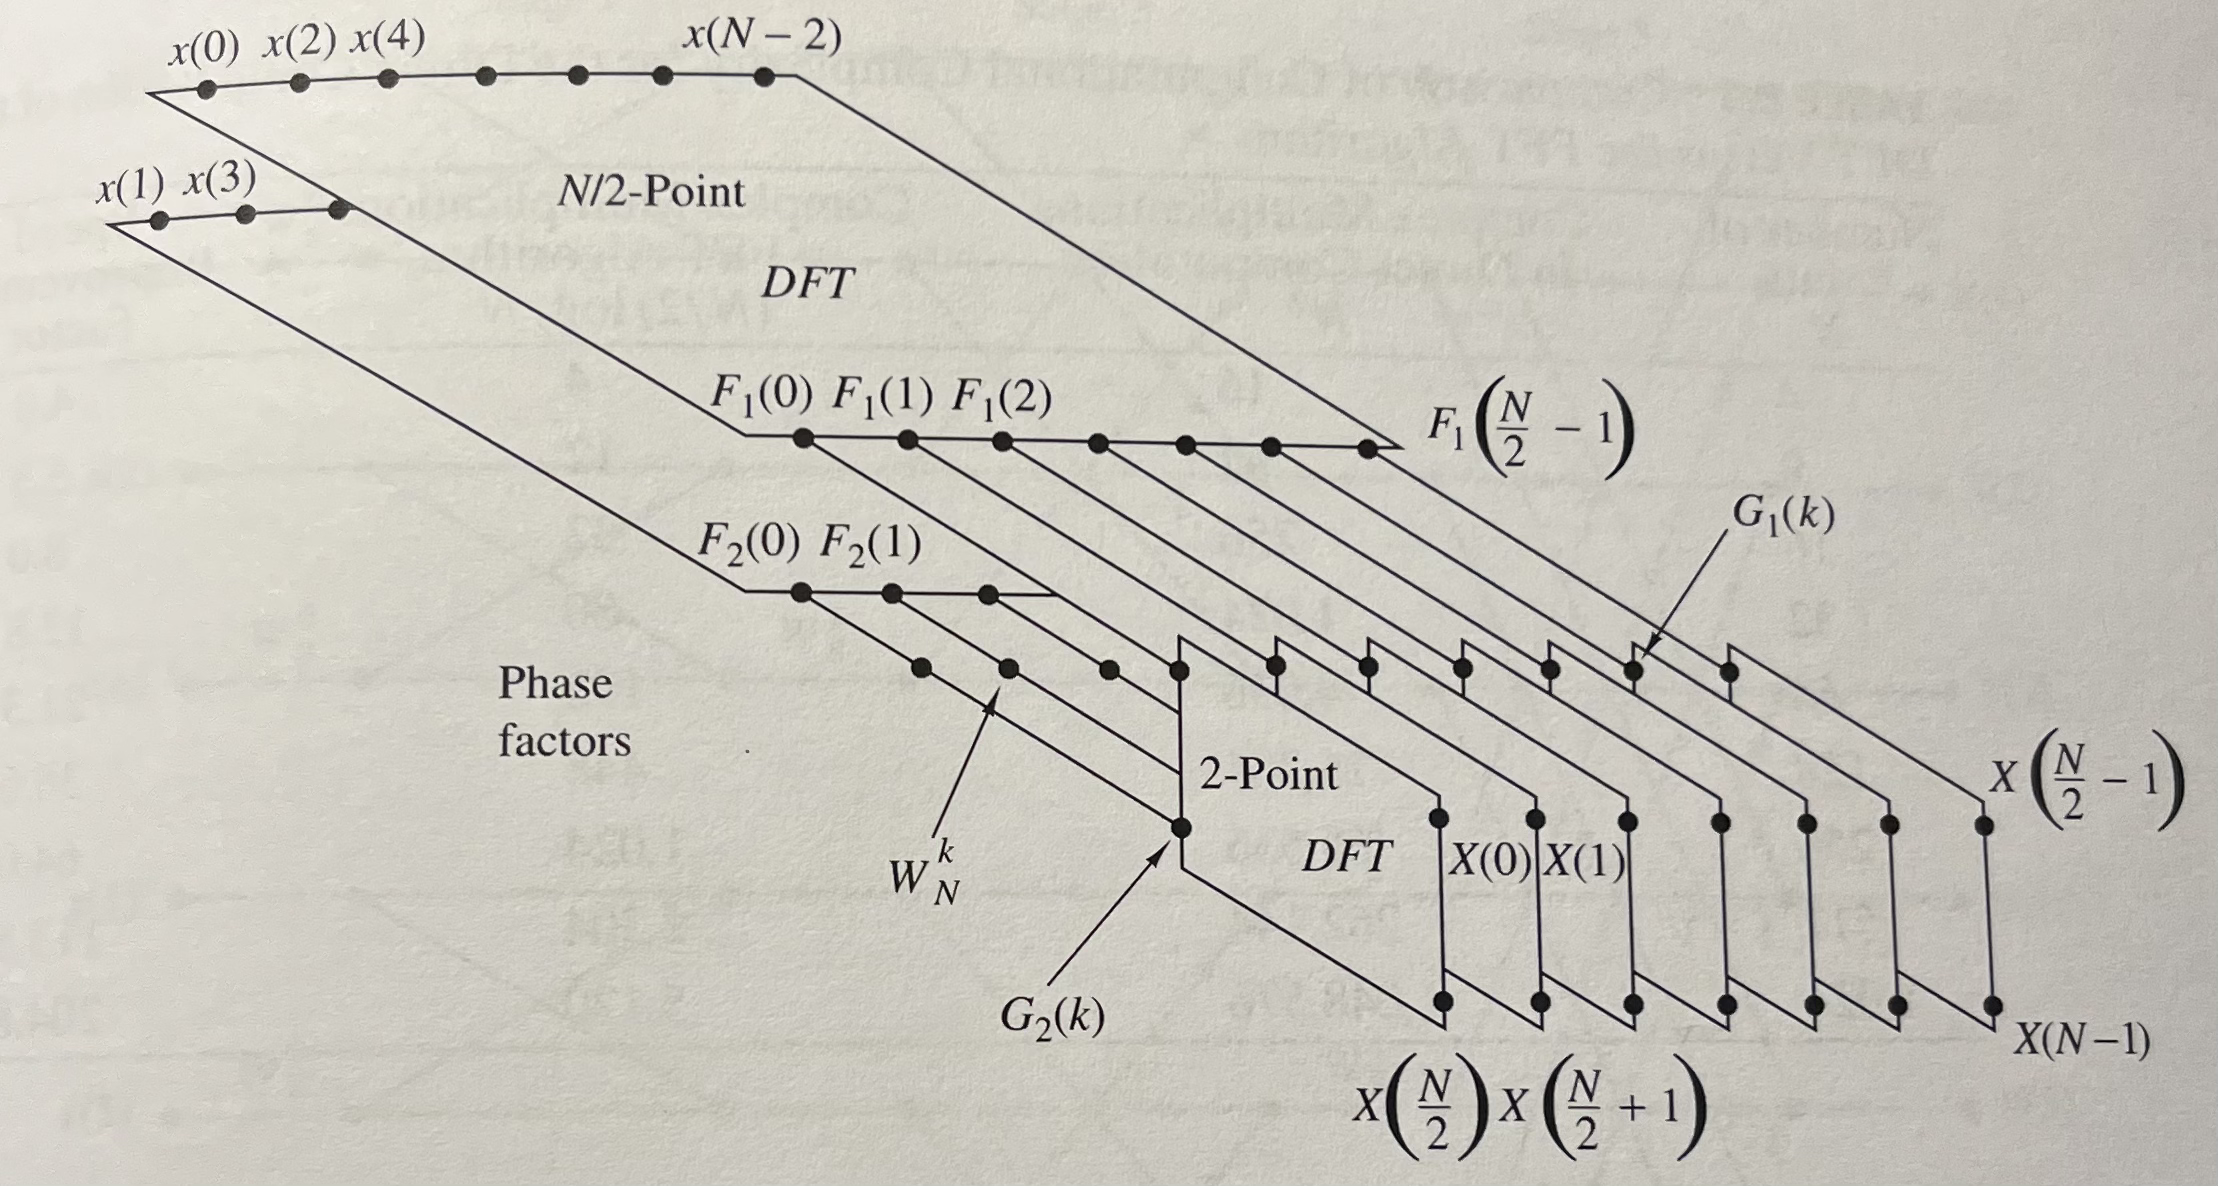
\includegraphics[width=10cm]{first_2}
	\caption{Two summation Radix 2}
	\end{figure}
	
	Figure 2 shows the an 8pt FFT using the radix-2 algorithm. 
	\begin{figure}[h]
	\centering
	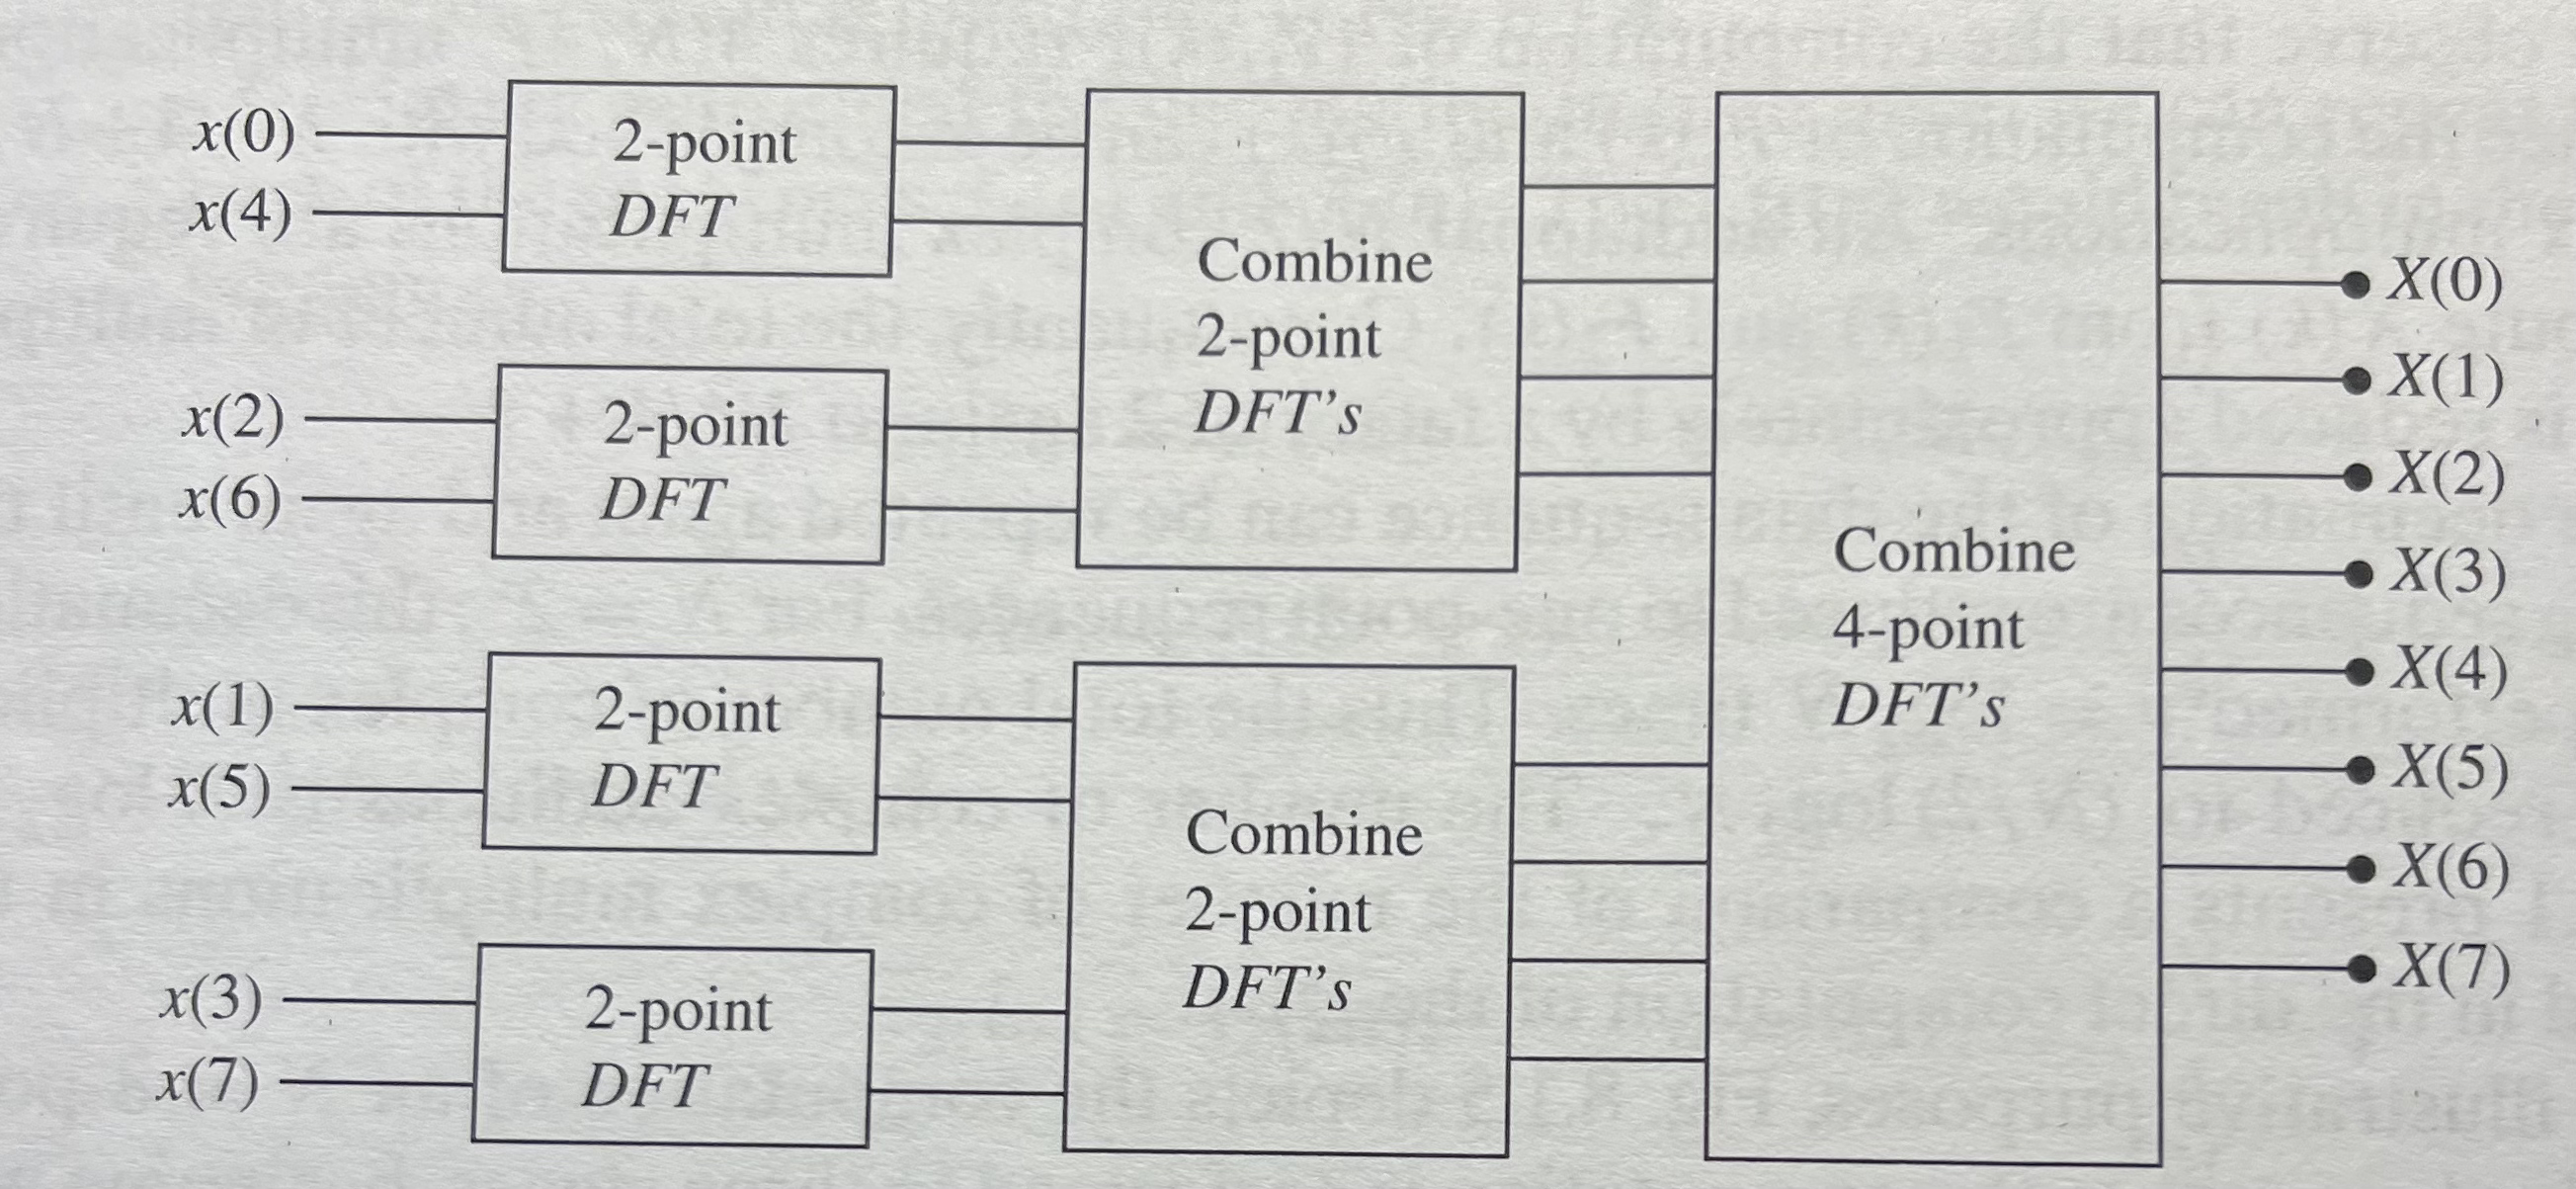
\includegraphics[width=10cm]{2pt}
	\caption{Radix 2 Algorithm}
	\end{figure}
	
	The butterfly unit is the main part of the FFT and is shown in figure 3. It includes a complex multiply and sum complex additions. 
	\begin{figure}[h]
	\centering
	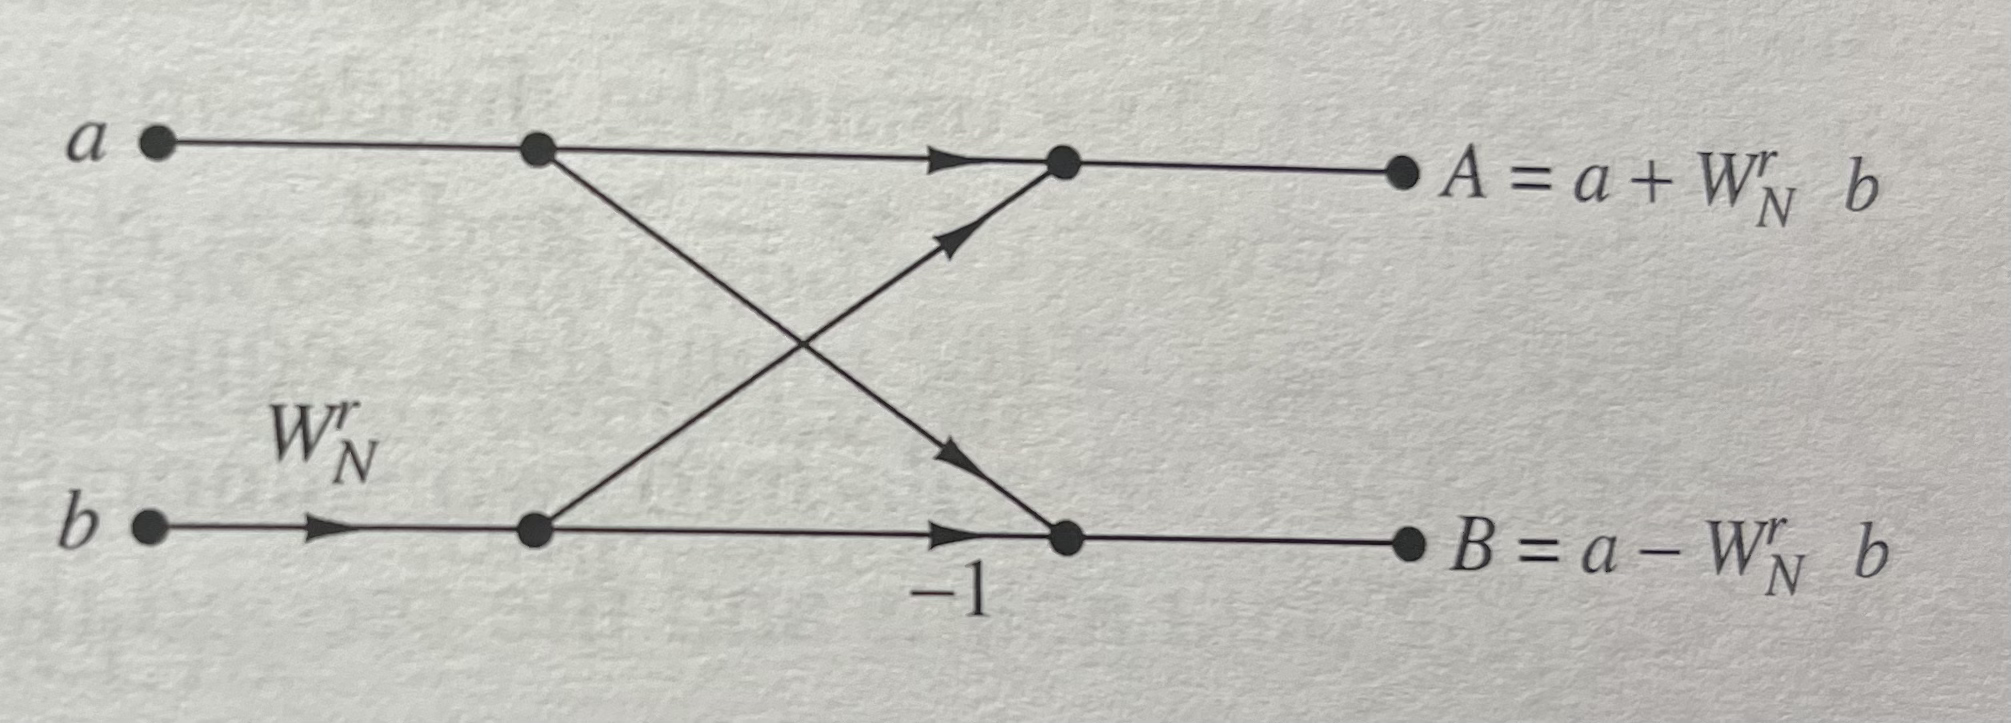
\includegraphics[width=10cm]{butterfly}
	\caption{Butterfly Unit}
	\end{figure}
	
	Figure 4 is the full algorithm for a 8-point Radix-2 algorithm with all the butterfly units. 
	\begin{figure}[h]
	\centering
	\includegraphics[width=7cm]{radix2}
	\caption{Full Radix 2 Algorithm}
	\end{figure}
	
	Figure 5 shows how you can reverse the bits and calculate the FFT in an algorithm.
	\begin{figure}[h]
	\centering
	\includegraphics[width=7cm]{bitflip}
	\caption{DIT Bitflip Algorithm}
	\end{figure}
	
	\subsection{Decimation in Frequency}
	In this section, first find $X(k)$ then decimate that in frequency the same way as it was done in time
	\begin{equation}
	X(2k) \text{ and } X(2k+1)
	\end{equation}
	
	Figure 6 e shows the Radix-2 Decimation in frequency algorithm.
	\begin{figure}[h]
	\centering
	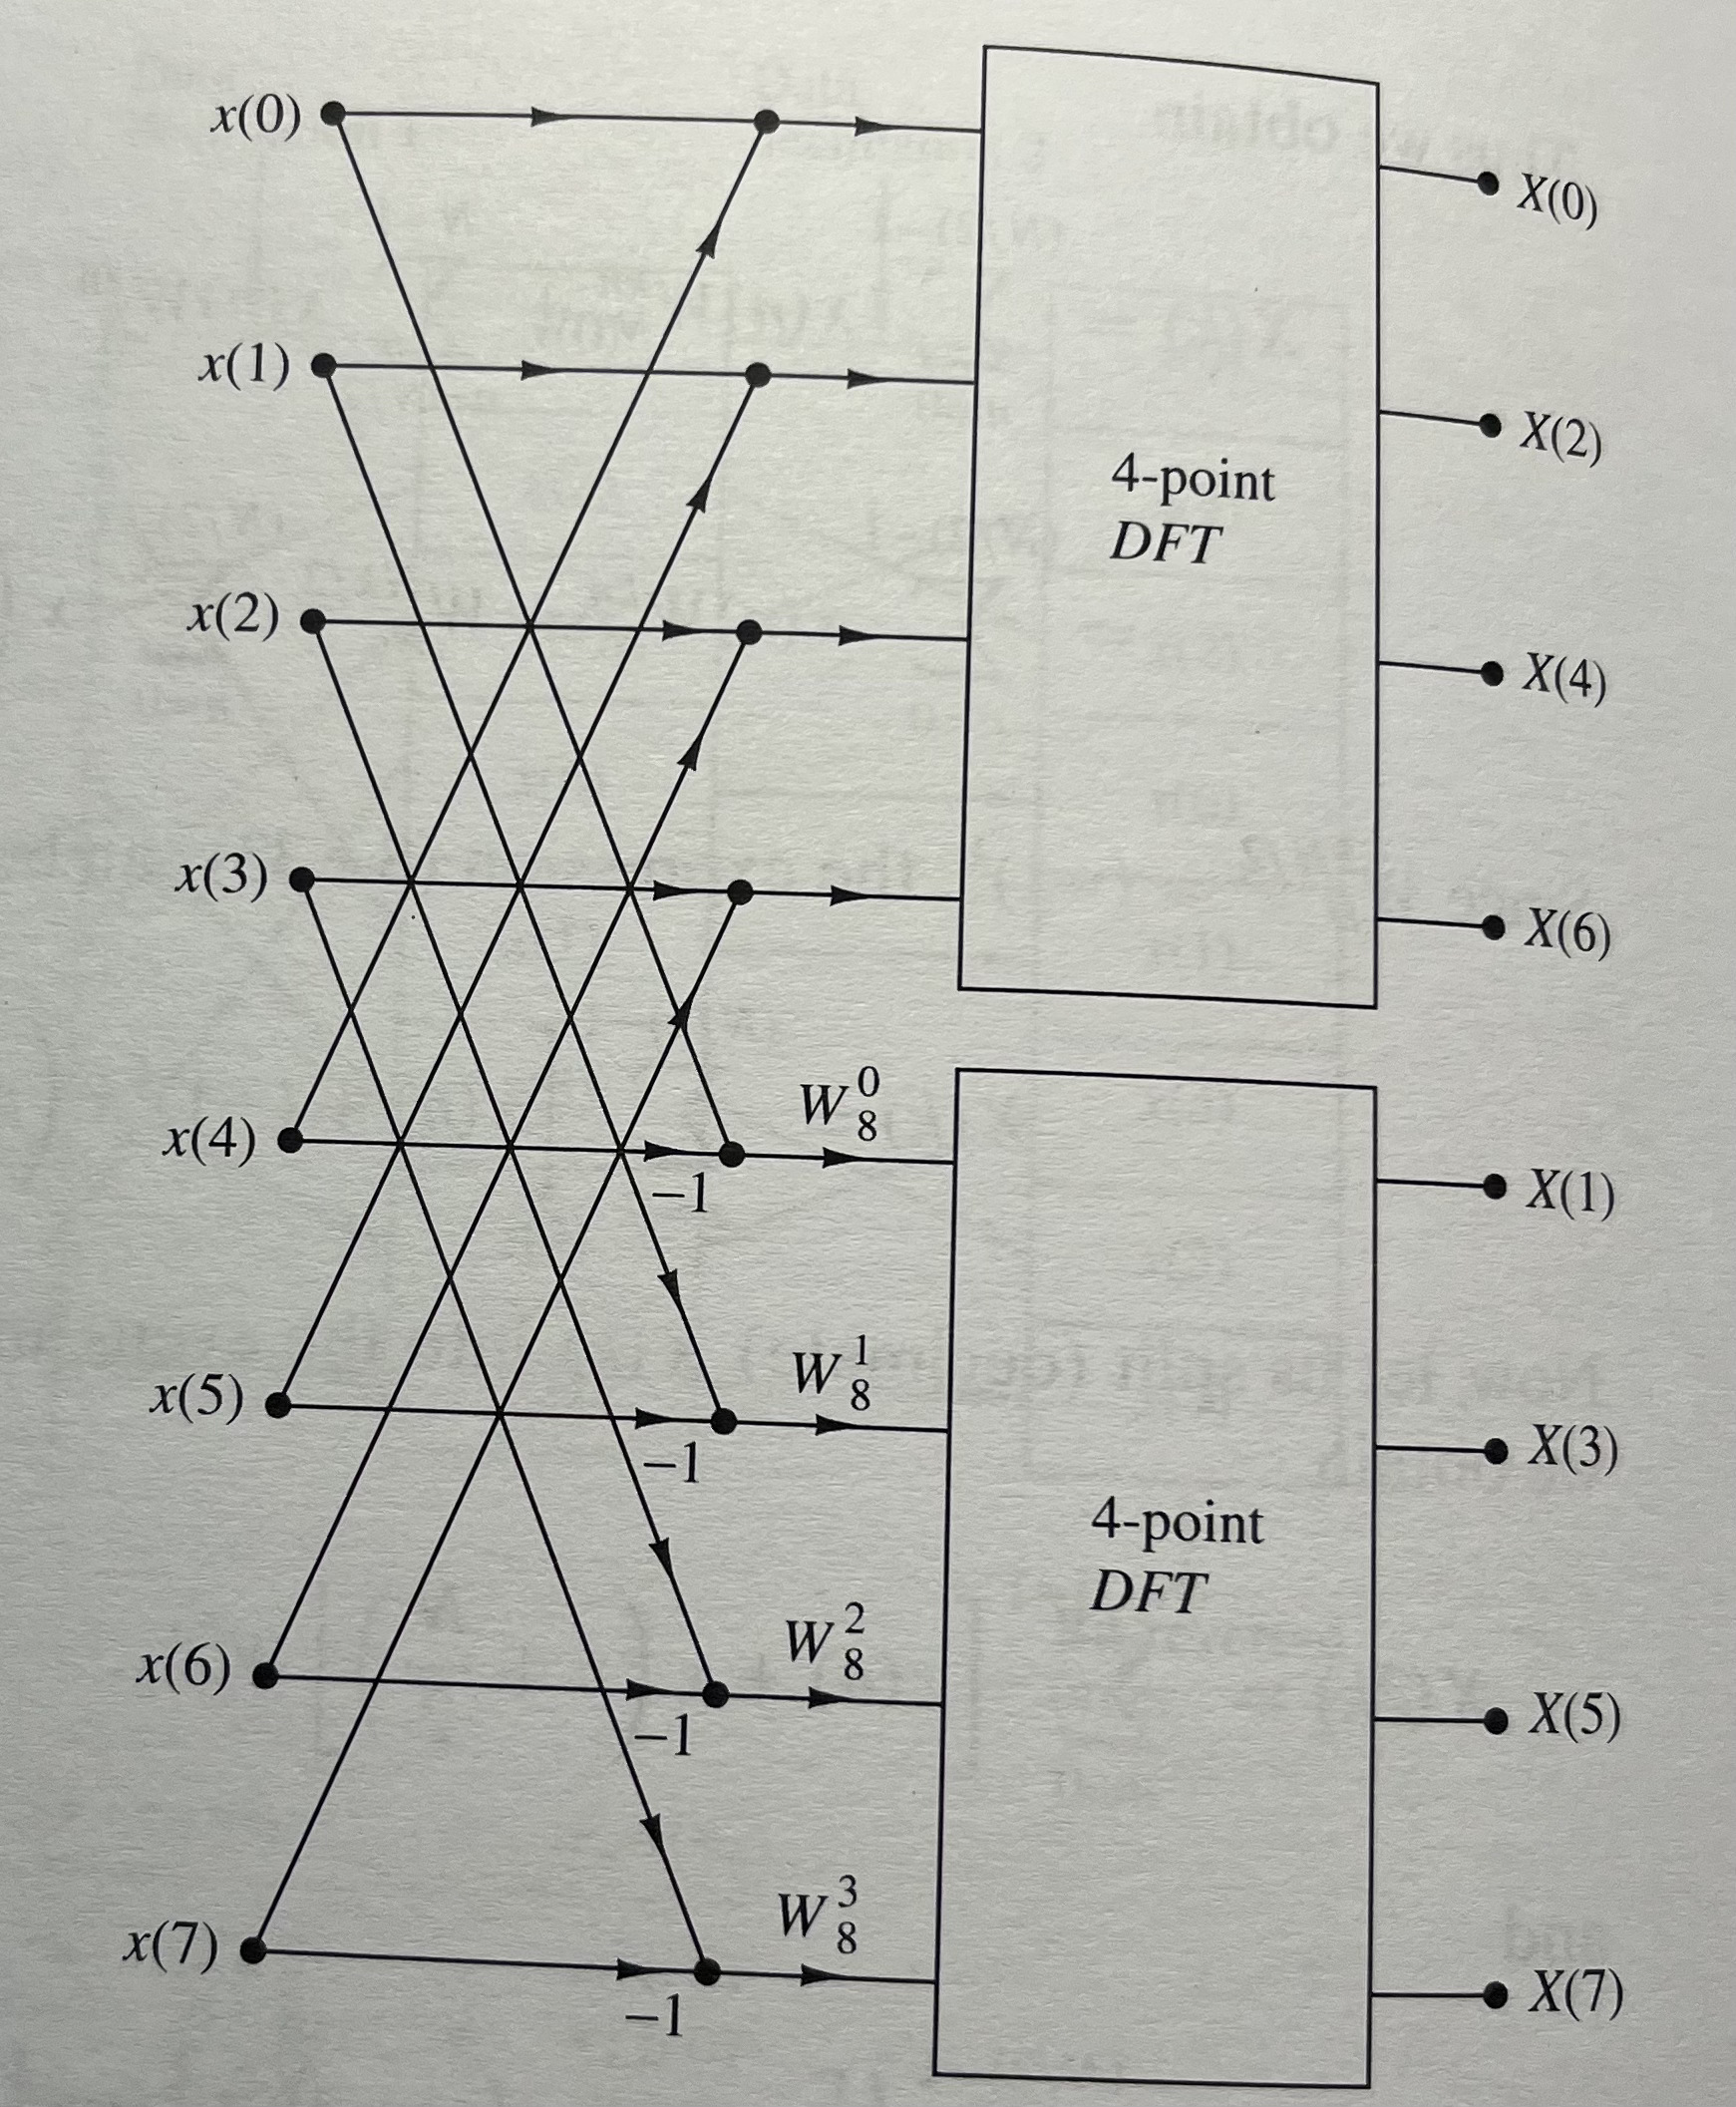
\includegraphics[width=7cm]{4pt}
	\caption{Radix-2 FFT DIF}
	\end{figure}
	
	\begin{figure}[h]
	\centering
	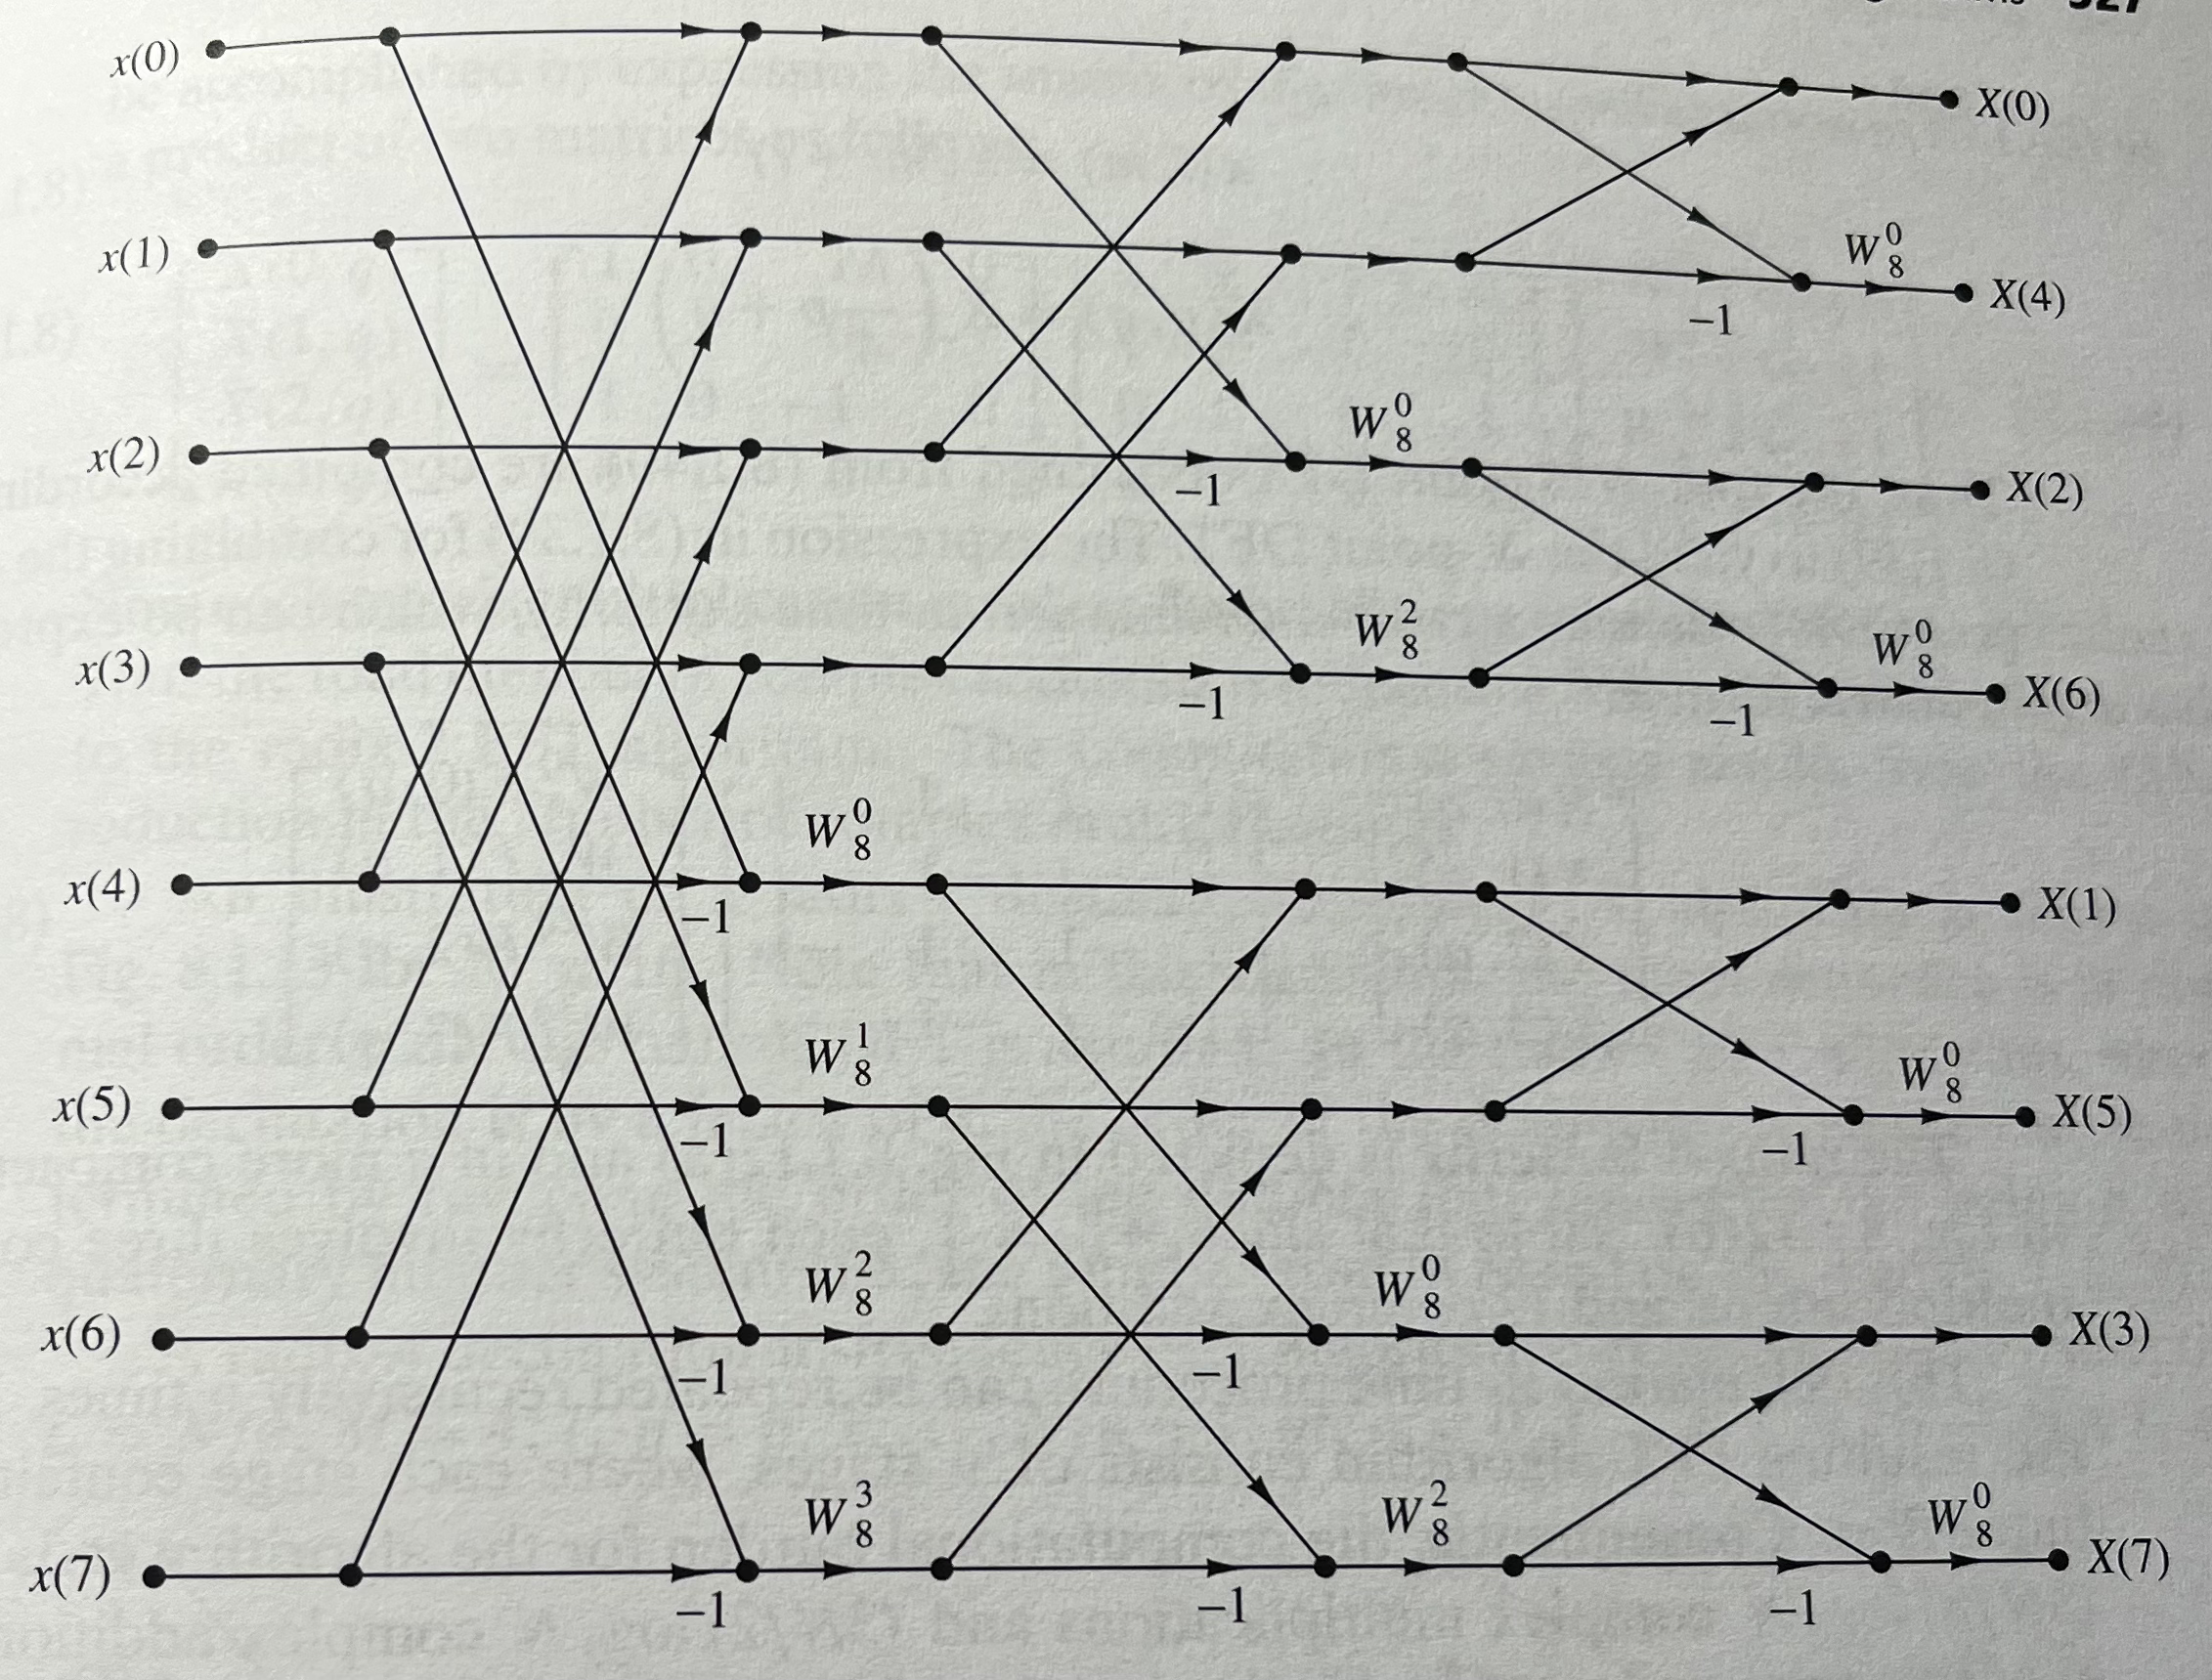
\includegraphics[width=10cm]{radix4}
	\caption{Full Radix-2 DIF Algorithm}
	\end{figure}

	
\end{document} % This is the end of the document